% Created by tikzDevice version 0.12.6 on 2026-08-08 02:45:02
% !TEX encoding = UTF-8 Unicode
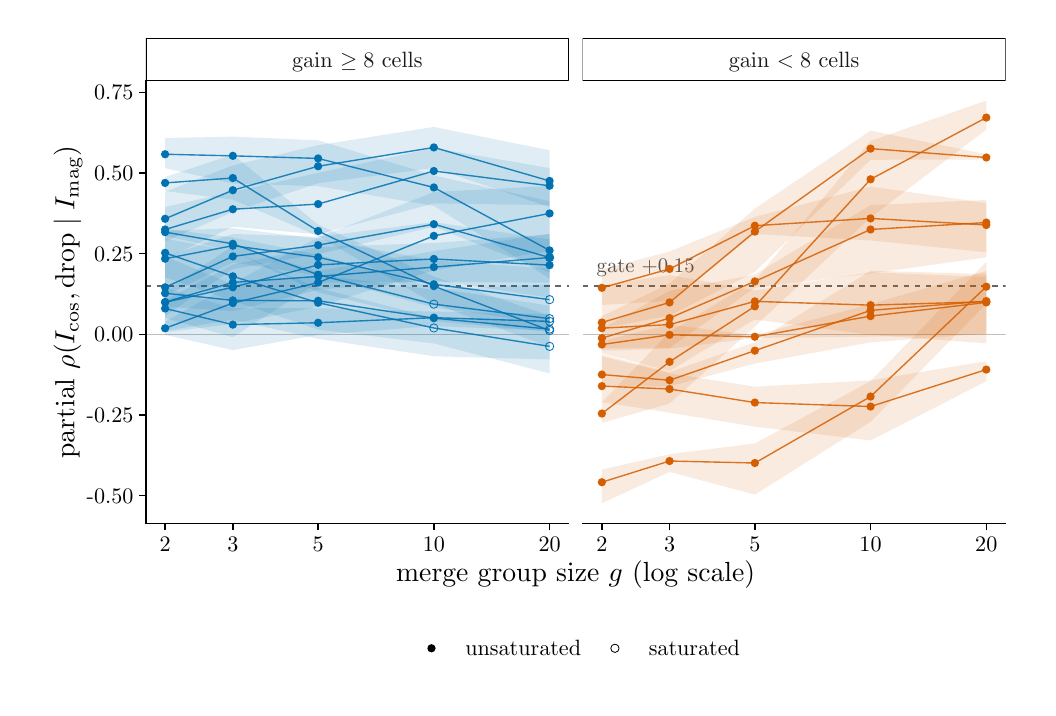
\begin{tikzpicture}[x=1pt,y=1pt]
\definecolor{fillColor}{RGB}{255,255,255}
\path[use as bounding box,fill=fillColor,fill opacity=0.00] (0,0) rectangle (361.35,238.49);
\begin{scope}
\path[clip] (  0.00,  0.00) rectangle (361.35,238.49);
\definecolor{drawColor}{RGB}{255,255,255}
\definecolor{fillColor}{RGB}{255,255,255}

\path[draw=drawColor,line width= 0.5pt,line join=round,line cap=round,fill=fillColor] (  0.00,  0.00) rectangle (361.35,238.49);
\end{scope}
\begin{scope}
\path[clip] ( 42.72, 59.35) rectangle (195.53,219.43);
\definecolor{fillColor}{RGB}{255,255,255}

\path[fill=fillColor] ( 42.72, 59.35) rectangle (195.53,219.43);
\definecolor{drawColor}{gray}{0.40}

\path[draw=drawColor,line width= 0.4pt,dash pattern=on 2pt off 2pt ,line join=round] ( 42.72,145.15) -- (195.53,145.15);
\definecolor{drawColor}{gray}{0.75}

\path[draw=drawColor,line width= 0.3pt,line join=round] ( 42.72,127.66) -- (195.53,127.66);
\definecolor{fillColor}{RGB}{0,114,178}

\path[fill=fillColor,fill opacity=0.12] ( 49.66,144.52) --
	( 74.13,137.13) --
	(104.95,137.10) --
	(146.77,135.88) --
	(188.59,135.07) --
	(188.59,129.05) --
	(146.77,130.68) --
	(104.95,127.49) --
	( 74.13,121.99) --
	( 49.66,127.50) --
	cycle;

\path[] ( 49.66,144.52) --
	( 74.13,137.13) --
	(104.95,137.10) --
	(146.77,135.88) --
	(188.59,135.07);

\path[] (188.59,129.05) --
	(146.77,130.68) --
	(104.95,127.49) --
	( 74.13,121.99) --
	( 49.66,127.50);

\path[fill=fillColor,fill opacity=0.12] ( 49.66,155.85) --
	( 74.13,145.68) --
	(104.95,149.13) --
	(146.77,143.76) --
	(188.59,145.75) --
	(188.59,118.58) --
	(146.77,119.76) --
	(104.95,126.05) --
	( 74.13,132.97) --
	( 49.66,128.93) --
	cycle;

\path[] ( 49.66,155.85) --
	( 74.13,145.68) --
	(104.95,149.13) --
	(146.77,143.76) --
	(188.59,145.75);

\path[] (188.59,118.58) --
	(146.77,119.76) --
	(104.95,126.05) --
	( 74.13,132.97) --
	( 49.66,128.93);

\path[fill=fillColor,fill opacity=0.12] ( 49.66,162.22) --
	( 74.13,157.80) --
	(104.95,144.44) --
	(146.77,133.59) --
	(188.59,132.44) --
	(188.59,113.56) --
	(146.77,124.37) --
	(104.95,129.38) --
	( 74.13,139.77) --
	( 49.66,148.29) --
	cycle;

\path[] ( 49.66,162.22) --
	( 74.13,157.80) --
	(104.95,144.44) --
	(146.77,133.59) --
	(188.59,132.44);

\path[] (188.59,113.56) --
	(146.77,124.37) --
	(104.95,129.38) --
	( 74.13,139.77) --
	( 49.66,148.29);

\path[fill=fillColor,fill opacity=0.12] ( 49.66,179.17) --
	( 74.13,188.73) --
	(104.95,196.01) --
	(146.77,202.61) --
	(188.59,194.18) --
	(188.59,173.60) --
	(146.77,187.80) --
	(104.95,182.31) --
	( 74.13,171.87) --
	( 49.66,161.20) --
	cycle;

\path[] ( 49.66,179.17) --
	( 74.13,188.73) --
	(104.95,196.01) --
	(146.77,202.61) --
	(188.59,194.18);

\path[] (188.59,173.60) --
	(146.77,187.80) --
	(104.95,182.31) --
	( 74.13,171.87) --
	( 49.66,161.20);

\path[fill=fillColor,fill opacity=0.12] ( 49.66,184.52) --
	( 74.13,192.63) --
	(104.95,167.33) --
	(146.77,148.57) --
	(188.59,134.40) --
	(188.59,123.07) --
	(146.77,138.82) --
	(104.95,163.21) --
	( 74.13,176.35) --
	( 49.66,179.47) --
	cycle;

\path[] ( 49.66,184.52) --
	( 74.13,192.63) --
	(104.95,167.33) --
	(146.77,148.57) --
	(188.59,134.40);

\path[] (188.59,123.07) --
	(146.77,138.82) --
	(104.95,163.21) --
	( 74.13,176.35) --
	( 49.66,179.47);

\path[fill=fillColor,fill opacity=0.12] ( 49.66,165.81) --
	( 74.13,162.67) --
	(104.95,156.42) --
	(146.77,144.49) --
	(188.59,138.01) --
	(188.59,128.58) --
	(146.77,132.53) --
	(104.95,142.90) --
	( 74.13,157.77) --
	( 49.66,163.25) --
	cycle;

\path[] ( 49.66,165.81) --
	( 74.13,162.67) --
	(104.95,156.42) --
	(146.77,144.49) --
	(188.59,138.01);

\path[] (188.59,128.58) --
	(146.77,132.53) --
	(104.95,142.90) --
	( 74.13,157.77) --
	( 49.66,163.25);

\path[fill=fillColor,fill opacity=0.12] ( 49.66,165.12) --
	( 74.13,166.03) --
	(104.95,162.23) --
	(146.77,154.36) --
	(188.59,151.43) --
	(188.59,131.67) --
	(146.77,137.34) --
	(104.95,148.93) --
	( 74.13,153.63) --
	( 49.66,141.59) --
	cycle;

\path[] ( 49.66,165.12) --
	( 74.13,166.03) --
	(104.95,162.23) --
	(146.77,154.36) --
	(188.59,151.43);

\path[] (188.59,131.67) --
	(146.77,137.34) --
	(104.95,148.93) --
	( 74.13,153.63) --
	( 49.66,141.59);

\path[fill=fillColor,fill opacity=0.12] ( 49.66,198.61) --
	( 74.13,199.11) --
	(104.95,197.79) --
	(146.77,185.08) --
	(188.59,175.77) --
	(188.59,147.81) --
	(146.77,174.11) --
	(104.95,181.21) --
	( 74.13,182.20) --
	( 49.66,187.74) --
	cycle;

\path[] ( 49.66,198.61) --
	( 74.13,199.11) --
	(104.95,197.79) --
	(146.77,185.08) --
	(188.59,175.77);

\path[] (188.59,147.81) --
	(146.77,174.11) --
	(104.95,181.21) --
	( 74.13,182.20) --
	( 49.66,187.74);

\path[fill=fillColor,fill opacity=0.12] ( 49.66,173.69) --
	( 74.13,179.18) --
	(104.95,186.02) --
	(146.77,195.01) --
	(188.59,187.74) --
	(188.59,174.37) --
	(146.77,175.01) --
	(104.95,163.81) --
	( 74.13,166.57) --
	( 49.66,154.92) --
	cycle;

\path[] ( 49.66,173.69) --
	( 74.13,179.18) --
	(104.95,186.02) --
	(146.77,195.01) --
	(188.59,187.74);

\path[] (188.59,174.37) --
	(146.77,175.01) --
	(104.95,163.81) --
	( 74.13,166.57) --
	( 49.66,154.92);

\path[fill=fillColor,fill opacity=0.12] ( 49.66,132.27) --
	( 74.13,146.10) --
	(104.95,162.67) --
	(146.77,179.08) --
	(188.59,181.28) --
	(188.59,157.89) --
	(146.77,150.82) --
	(104.95,137.71) --
	( 74.13,131.48) --
	( 49.66,128.40) --
	cycle;

\path[] ( 49.66,132.27) --
	( 74.13,146.10) --
	(104.95,162.67) --
	(146.77,179.08) --
	(188.59,181.28);

\path[] (188.59,157.89) --
	(146.77,150.82) --
	(104.95,137.71) --
	( 74.13,131.48) --
	( 49.66,128.40);

\path[fill=fillColor,fill opacity=0.12] ( 49.66,140.09) --
	( 74.13,152.90) --
	(104.95,159.24) --
	(146.77,160.65) --
	(188.59,163.85) --
	(188.59,140.91) --
	(146.77,147.29) --
	(104.95,143.78) --
	( 74.13,136.09) --
	( 49.66,137.67) --
	cycle;

\path[] ( 49.66,140.09) --
	( 74.13,152.90) --
	(104.95,159.24) --
	(146.77,160.65) --
	(188.59,163.85);

\path[] (188.59,140.91) --
	(146.77,147.29) --
	(104.95,143.78) --
	( 74.13,136.09) --
	( 49.66,137.67);

\path[fill=fillColor,fill opacity=0.12] ( 49.66,155.73) --
	( 74.13,163.94) --
	(104.95,162.94) --
	(146.77,168.21) --
	(188.59,161.98) --
	(188.59,149.97) --
	(146.77,166.60) --
	(104.95,156.61) --
	( 74.13,151.27) --
	( 49.66,134.30) --
	cycle;

\path[] ( 49.66,155.73) --
	( 74.13,163.94) --
	(104.95,162.94) --
	(146.77,168.21) --
	(188.59,161.98);

\path[] (188.59,149.97) --
	(146.77,166.60) --
	(104.95,156.61) --
	( 74.13,151.27) --
	( 49.66,134.30);

\path[fill=fillColor,fill opacity=0.12] ( 49.66,143.07) --
	( 74.13,159.64) --
	(104.95,150.58) --
	(146.77,157.75) --
	(188.59,164.03) --
	(188.59,146.33) --
	(146.77,146.69) --
	(104.95,146.38) --
	( 74.13,126.65) --
	( 49.66,133.56) --
	cycle;

\path[] ( 49.66,143.07) --
	( 74.13,159.64) --
	(104.95,150.58) --
	(146.77,157.75) --
	(188.59,164.03);

\path[] (188.59,146.33) --
	(146.77,146.69) --
	(104.95,146.38) --
	( 74.13,126.65) --
	( 49.66,133.56);
\definecolor{drawColor}{RGB}{0,114,178}

\path[draw=drawColor,draw opacity=0.85,line width= 0.5pt,line join=round] ( 49.66,137.01) --
	( 74.13,131.19) --
	(104.95,131.86) --
	(146.77,133.70) --
	(188.59,132.36);

\path[draw=drawColor,draw opacity=0.85,line width= 0.5pt,line join=round] ( 49.66,142.52) --
	( 74.13,139.95) --
	(104.95,139.79) --
	(146.77,133.52) --
	(188.59,129.56);

\path[draw=drawColor,draw opacity=0.85,line width= 0.5pt,line join=round] ( 49.66,157.12) --
	( 74.13,148.64) --
	(104.95,139.09) --
	(146.77,129.98) --
	(188.59,123.32);

\path[draw=drawColor,draw opacity=0.85,line width= 0.5pt,line join=round] ( 49.66,169.43) --
	( 74.13,179.76) --
	(104.95,188.41) --
	(146.77,195.21) --
	(188.59,183.11);

\path[draw=drawColor,draw opacity=0.85,line width= 0.5pt,line join=round] ( 49.66,182.39) --
	( 74.13,184.16) --
	(104.95,165.01) --
	(146.77,145.10) --
	(188.59,129.05);

\path[draw=drawColor,draw opacity=0.85,line width= 0.5pt,line join=round] ( 49.66,164.61) --
	( 74.13,160.38) --
	(104.95,149.24) --
	(146.77,138.58) --
	(188.59,133.35);

\path[draw=drawColor,draw opacity=0.85,line width= 0.5pt,line join=round] ( 49.66,155.00) --
	( 74.13,159.70) --
	(104.95,155.53) --
	(146.77,145.77) --
	(188.59,140.21);

\path[draw=drawColor,draw opacity=0.85,line width= 0.5pt,line join=round] ( 49.66,192.75) --
	( 74.13,192.17) --
	(104.95,191.24) --
	(146.77,180.74) --
	(188.59,158.00);

\path[draw=drawColor,draw opacity=0.85,line width= 0.5pt,line join=round] ( 49.66,165.56) --
	( 74.13,172.88) --
	(104.95,174.75) --
	(146.77,186.69) --
	(188.59,181.36);

\path[draw=drawColor,draw opacity=0.85,line width= 0.5pt,line join=round] ( 49.66,129.86) --
	( 74.13,138.96) --
	(104.95,146.38) --
	(146.77,163.26) --
	(188.59,171.37);

\path[draw=drawColor,draw opacity=0.85,line width= 0.5pt,line join=round] ( 49.66,139.26) --
	( 74.13,144.68) --
	(104.95,152.76) --
	(146.77,154.92) --
	(188.59,152.69);

\path[draw=drawColor,draw opacity=0.85,line width= 0.5pt,line join=round] ( 49.66,144.66) --
	( 74.13,155.83) --
	(104.95,159.90) --
	(146.77,167.48) --
	(188.59,155.42);

\path[draw=drawColor,draw opacity=0.85,line width= 0.5pt,line join=round] ( 49.66,139.36) --
	( 74.13,146.42) --
	(104.95,148.60) --
	(146.77,151.96) --
	(188.59,155.44);
\definecolor{fillColor}{RGB}{0,114,178}

\path[fill=fillColor] ( 49.66,169.43) circle (  1.50);

\path[fill=fillColor] ( 74.13,179.76) circle (  1.50);

\path[fill=fillColor] (104.95,188.41) circle (  1.50);

\path[fill=fillColor] (146.77,195.21) circle (  1.50);

\path[fill=fillColor] (188.59,183.11) circle (  1.50);

\path[fill=fillColor] ( 49.66,182.39) circle (  1.50);

\path[fill=fillColor] ( 74.13,184.16) circle (  1.50);

\path[fill=fillColor] (104.95,165.01) circle (  1.50);

\path[fill=fillColor] (146.77,145.10) circle (  1.50);
\definecolor{drawColor}{RGB}{0,114,178}

\path[draw=drawColor,line width= 0.3pt,line join=round,line cap=round] (188.59,129.05) circle (  1.50);

\path[fill=fillColor] ( 49.66,164.61) circle (  1.50);

\path[fill=fillColor] ( 74.13,160.38) circle (  1.50);

\path[fill=fillColor] (104.95,149.24) circle (  1.50);

\path[draw=drawColor,line width= 0.3pt,line join=round,line cap=round] (146.77,138.58) circle (  1.50);

\path[draw=drawColor,line width= 0.3pt,line join=round,line cap=round] (188.59,133.35) circle (  1.50);

\path[fill=fillColor] ( 49.66,155.00) circle (  1.50);

\path[fill=fillColor] ( 74.13,159.70) circle (  1.50);

\path[fill=fillColor] (104.95,155.53) circle (  1.50);

\path[fill=fillColor] (146.77,145.77) circle (  1.50);

\path[draw=drawColor,line width= 0.3pt,line join=round,line cap=round] (188.59,140.21) circle (  1.50);

\path[fill=fillColor] ( 49.66,192.75) circle (  1.50);

\path[fill=fillColor] ( 74.13,192.17) circle (  1.50);

\path[fill=fillColor] (104.95,191.24) circle (  1.50);

\path[fill=fillColor] (146.77,180.74) circle (  1.50);

\path[fill=fillColor] (188.59,158.00) circle (  1.50);

\path[fill=fillColor] ( 49.66,165.56) circle (  1.50);

\path[fill=fillColor] ( 74.13,172.88) circle (  1.50);

\path[fill=fillColor] (104.95,174.75) circle (  1.50);

\path[fill=fillColor] (146.77,186.69) circle (  1.50);

\path[fill=fillColor] (188.59,181.36) circle (  1.50);

\path[fill=fillColor] ( 49.66,129.86) circle (  1.50);

\path[fill=fillColor] ( 74.13,138.96) circle (  1.50);

\path[fill=fillColor] (104.95,146.38) circle (  1.50);

\path[fill=fillColor] (146.77,163.26) circle (  1.50);

\path[fill=fillColor] (188.59,171.37) circle (  1.50);

\path[fill=fillColor] ( 49.66,139.26) circle (  1.50);

\path[fill=fillColor] ( 74.13,144.68) circle (  1.50);

\path[fill=fillColor] (104.95,152.76) circle (  1.50);

\path[fill=fillColor] (146.77,154.92) circle (  1.50);

\path[fill=fillColor] (188.59,152.69) circle (  1.50);

\path[fill=fillColor] ( 49.66,144.66) circle (  1.50);

\path[fill=fillColor] ( 74.13,155.83) circle (  1.50);

\path[fill=fillColor] (104.95,159.90) circle (  1.50);

\path[fill=fillColor] (146.77,167.48) circle (  1.50);

\path[draw=drawColor,line width= 0.3pt,line join=round,line cap=round] (188.59,155.42) circle (  1.50);

\path[fill=fillColor] ( 49.66,139.36) circle (  1.50);

\path[fill=fillColor] ( 74.13,146.42) circle (  1.50);

\path[fill=fillColor] (104.95,148.60) circle (  1.50);

\path[fill=fillColor] (146.77,151.96) circle (  1.50);

\path[fill=fillColor] (188.59,155.44) circle (  1.50);

\path[fill=fillColor] ( 49.66,137.01) circle (  1.50);

\path[fill=fillColor] ( 74.13,131.19) circle (  1.50);

\path[fill=fillColor] (104.95,131.86) circle (  1.50);

\path[fill=fillColor] (146.77,133.70) circle (  1.50);

\path[draw=drawColor,line width= 0.3pt,line join=round,line cap=round] (188.59,132.36) circle (  1.50);

\path[fill=fillColor] ( 49.66,142.52) circle (  1.50);

\path[fill=fillColor] ( 74.13,139.95) circle (  1.50);

\path[fill=fillColor] (104.95,139.79) circle (  1.50);

\path[fill=fillColor] (146.77,133.52) circle (  1.50);

\path[draw=drawColor,line width= 0.3pt,line join=round,line cap=round] (188.59,129.56) circle (  1.50);

\path[fill=fillColor] ( 49.66,157.12) circle (  1.50);

\path[fill=fillColor] ( 74.13,148.64) circle (  1.50);

\path[fill=fillColor] (104.95,139.09) circle (  1.50);

\path[draw=drawColor,line width= 0.3pt,line join=round,line cap=round] (146.77,129.98) circle (  1.50);

\path[draw=drawColor,line width= 0.3pt,line join=round,line cap=round] (188.59,123.32) circle (  1.50);
\end{scope}
\begin{scope}
\path[clip] (200.53, 59.35) rectangle (353.35,219.43);
\definecolor{fillColor}{RGB}{255,255,255}

\path[fill=fillColor] (200.53, 59.35) rectangle (353.35,219.43);
\definecolor{drawColor}{gray}{0.40}

\path[draw=drawColor,line width= 0.4pt,dash pattern=on 2pt off 2pt ,line join=round] (200.53,145.15) -- (353.35,145.15);
\definecolor{drawColor}{gray}{0.75}

\path[draw=drawColor,line width= 0.3pt,line join=round] (200.53,127.66) -- (353.35,127.66);
\definecolor{drawColor}{gray}{0.30}

\node[text=drawColor,anchor=base,inner sep=0pt, outer sep=0pt, scale=  0.75] at (223.31,150.14) {gate $+0.15$};
\definecolor{fillColor}{RGB}{213,94,0}

\path[fill=fillColor,fill opacity=0.12] (207.48,145.39) --
	(231.94,149.10) --
	(262.76,143.53) --
	(304.58,150.12) --
	(346.40,148.42) --
	(346.40,124.43) --
	(304.58,127.49) --
	(262.76,133.04) --
	(231.94,114.43) --
	(207.48,120.81) --
	cycle;

\path[] (207.48,145.39) --
	(231.94,149.10) --
	(262.76,143.53) --
	(304.58,150.12) --
	(346.40,148.42);

\path[] (346.40,124.43) --
	(304.58,127.49) --
	(262.76,133.04) --
	(231.94,114.43) --
	(207.48,120.81);

\path[fill=fillColor,fill opacity=0.12] (207.48,120.41) --
	(231.94,114.04) --
	(262.76,124.83) --
	(304.58,150.67) --
	(346.40,149.47) --
	(346.40,128.00) --
	(304.58,124.79) --
	(262.76,117.10) --
	(231.94,108.90) --
	(207.48,108.96) --
	cycle;

\path[] (207.48,120.41) --
	(231.94,114.04) --
	(262.76,124.83) --
	(304.58,150.67) --
	(346.40,149.47);

\path[] (346.40,128.00) --
	(304.58,124.79) --
	(262.76,117.10) --
	(231.94,108.90) --
	(207.48,108.96);

\path[fill=fillColor,fill opacity=0.12] (207.48,119.72) --
	(231.94,113.63) --
	(262.76,108.75) --
	(304.58,111.02) --
	(346.40,117.98) --
	(346.40,110.71) --
	(304.58, 89.33) --
	(262.76, 94.31) --
	(231.94, 99.36) --
	(207.48,103.16) --
	cycle;

\path[] (207.48,119.72) --
	(231.94,113.63) --
	(262.76,108.75) --
	(304.58,111.02) --
	(346.40,117.98);

\path[] (346.40,110.71) --
	(304.58, 89.33) --
	(262.76, 94.31) --
	(231.94, 99.36) --
	(207.48,103.16);

\path[fill=fillColor,fill opacity=0.12] (207.48,103.13) --
	(231.94,128.47) --
	(262.76,147.15) --
	(304.58,197.55) --
	(346.40,212.15) --
	(346.40,201.64) --
	(304.58,169.91) --
	(262.76,130.47) --
	(231.94,102.68) --
	(207.48, 95.65) --
	cycle;

\path[] (207.48,103.13) --
	(231.94,128.47) --
	(262.76,147.15) --
	(304.58,197.55) --
	(346.40,212.15);

\path[] (346.40,201.64) --
	(304.58,169.91) --
	(262.76,130.47) --
	(231.94,102.68) --
	(207.48, 95.65);

\path[fill=fillColor,fill opacity=0.12] (207.48,129.67) --
	(231.94,143.43) --
	(262.76,149.29) --
	(304.58,174.39) --
	(346.40,176.24) --
	(346.40,155.51) --
	(304.58,149.70) --
	(262.76,144.51) --
	(231.94,122.78) --
	(207.48,122.58) --
	cycle;

\path[] (207.48,129.67) --
	(231.94,143.43) --
	(262.76,149.29) --
	(304.58,174.39) --
	(346.40,176.24);

\path[] (346.40,155.51) --
	(304.58,149.70) --
	(262.76,144.51) --
	(231.94,122.78) --
	(207.48,122.58);

\path[fill=fillColor,fill opacity=0.12] (207.48,125.23) --
	(231.94,131.18) --
	(262.76,127.34) --
	(304.58,138.60) --
	(346.40,150.58) --
	(346.40,127.81) --
	(304.58,126.82) --
	(262.76,126.38) --
	(231.94,122.52) --
	(207.48,121.76) --
	cycle;

\path[] (207.48,125.23) --
	(231.94,131.18) --
	(262.76,127.34) --
	(304.58,138.60) --
	(346.40,150.58);

\path[] (346.40,127.81) --
	(304.58,126.82) --
	(262.76,126.38) --
	(231.94,122.52) --
	(207.48,121.76);

\path[fill=fillColor,fill opacity=0.12] (207.48, 78.82) --
	(231.94, 84.34) --
	(262.76, 88.27) --
	(304.58,110.76) --
	(346.40,153.87) --
	(346.40,138.74) --
	(304.58, 96.05) --
	(262.76, 69.77) --
	(231.94, 77.97) --
	(207.48, 66.63) --
	cycle;

\path[] (207.48, 78.82) --
	(231.94, 84.34) --
	(262.76, 88.27) --
	(304.58,110.76) --
	(346.40,153.87);

\path[] (346.40,138.74) --
	(304.58, 96.05) --
	(262.76, 69.77) --
	(231.94, 77.97) --
	(207.48, 66.63);

\path[fill=fillColor,fill opacity=0.12] (207.48,134.22) --
	(231.94,146.05) --
	(262.76,173.10) --
	(304.58,201.28) --
	(346.40,192.73) --
	(346.40,190.82) --
	(304.58,190.75) --
	(262.76,150.24) --
	(231.94,134.41) --
	(207.48,129.95) --
	cycle;

\path[] (207.48,134.22) --
	(231.94,146.05) --
	(262.76,173.10) --
	(304.58,201.28) --
	(346.40,192.73);

\path[] (346.40,190.82) --
	(304.58,190.75) --
	(262.76,150.24) --
	(231.94,134.41) --
	(207.48,129.95);

\path[fill=fillColor,fill opacity=0.12] (207.48,151.18) --
	(231.94,157.62) --
	(262.76,170.11) --
	(304.58,181.07) --
	(346.40,175.14) --
	(346.40,157.34) --
	(304.58,161.59) --
	(262.76,163.95) --
	(231.94,139.77) --
	(207.48,138.27) --
	cycle;

\path[] (207.48,151.18) --
	(231.94,157.62) --
	(262.76,170.11) --
	(304.58,181.07) --
	(346.40,175.14);

\path[] (346.40,157.34) --
	(304.58,161.59) --
	(262.76,163.95) --
	(231.94,139.77) --
	(207.48,138.27);
\definecolor{drawColor}{RGB}{213,94,0}

\path[draw=drawColor,draw opacity=0.85,line width= 0.5pt,line join=round] (207.48,129.90) --
	(231.94,131.20) --
	(262.76,139.59) --
	(304.58,138.22) --
	(346.40,139.47);

\path[draw=drawColor,draw opacity=0.85,line width= 0.5pt,line join=round] (207.48,113.14) --
	(231.94,111.08) --
	(262.76,121.78) --
	(304.58,136.33) --
	(346.40,139.68);

\path[draw=drawColor,draw opacity=0.85,line width= 0.5pt,line join=round] (207.48,108.97) --
	(231.94,107.91) --
	(262.76,103.02) --
	(304.58,101.59) --
	(346.40,114.94);

\path[draw=drawColor,draw opacity=0.85,line width= 0.5pt,line join=round] (207.48, 99.05) --
	(231.94,117.75) --
	(262.76,137.79) --
	(304.58,183.70) --
	(346.40,206.00);

\path[draw=drawColor,draw opacity=0.85,line width= 0.5pt,line join=round] (207.48,126.31) --
	(231.94,133.54) --
	(262.76,146.81) --
	(304.58,165.57) --
	(346.40,168.07);

\path[draw=drawColor,draw opacity=0.85,line width= 0.5pt,line join=round] (207.48,124.00) --
	(231.94,127.50) --
	(262.76,126.80) --
	(304.58,134.26) --
	(346.40,139.21);

\path[draw=drawColor,draw opacity=0.85,line width= 0.5pt,line join=round] (207.48, 74.24) --
	(231.94, 81.90) --
	(262.76, 81.18) --
	(304.58,105.20) --
	(346.40,144.90);

\path[draw=drawColor,draw opacity=0.85,line width= 0.5pt,line join=round] (207.48,131.95) --
	(231.94,139.20) --
	(262.76,164.80) --
	(304.58,194.79) --
	(346.40,191.57);

\path[draw=drawColor,draw opacity=0.85,line width= 0.5pt,line join=round] (207.48,144.48) --
	(231.94,151.31) --
	(262.76,166.93) --
	(304.58,169.56) --
	(346.40,167.18);
\definecolor{fillColor}{RGB}{213,94,0}

\path[fill=fillColor] (207.48, 99.05) circle (  1.50);

\path[fill=fillColor] (231.94,117.75) circle (  1.50);

\path[fill=fillColor] (262.76,137.79) circle (  1.50);

\path[fill=fillColor] (304.58,183.70) circle (  1.50);

\path[fill=fillColor] (346.40,206.00) circle (  1.50);

\path[fill=fillColor] (207.48,126.31) circle (  1.50);

\path[fill=fillColor] (231.94,133.54) circle (  1.50);

\path[fill=fillColor] (262.76,146.81) circle (  1.50);

\path[fill=fillColor] (304.58,165.57) circle (  1.50);

\path[fill=fillColor] (346.40,168.07) circle (  1.50);

\path[fill=fillColor] (207.48,124.00) circle (  1.50);

\path[fill=fillColor] (231.94,127.50) circle (  1.50);

\path[fill=fillColor] (262.76,126.80) circle (  1.50);

\path[fill=fillColor] (304.58,134.26) circle (  1.50);

\path[fill=fillColor] (346.40,139.21) circle (  1.50);

\path[fill=fillColor] (207.48, 74.24) circle (  1.50);

\path[fill=fillColor] (231.94, 81.90) circle (  1.50);

\path[fill=fillColor] (262.76, 81.18) circle (  1.50);

\path[fill=fillColor] (304.58,105.20) circle (  1.50);

\path[fill=fillColor] (346.40,144.90) circle (  1.50);

\path[fill=fillColor] (207.48,131.95) circle (  1.50);

\path[fill=fillColor] (231.94,139.20) circle (  1.50);

\path[fill=fillColor] (262.76,164.80) circle (  1.50);

\path[fill=fillColor] (304.58,194.79) circle (  1.50);

\path[fill=fillColor] (346.40,191.57) circle (  1.50);

\path[fill=fillColor] (207.48,144.48) circle (  1.50);

\path[fill=fillColor] (231.94,151.31) circle (  1.50);

\path[fill=fillColor] (262.76,166.93) circle (  1.50);

\path[fill=fillColor] (304.58,169.56) circle (  1.50);

\path[fill=fillColor] (346.40,167.18) circle (  1.50);

\path[fill=fillColor] (207.48,129.90) circle (  1.50);

\path[fill=fillColor] (231.94,131.20) circle (  1.50);

\path[fill=fillColor] (262.76,139.59) circle (  1.50);

\path[fill=fillColor] (304.58,138.22) circle (  1.50);

\path[fill=fillColor] (346.40,139.47) circle (  1.50);

\path[fill=fillColor] (207.48,113.14) circle (  1.50);

\path[fill=fillColor] (231.94,111.08) circle (  1.50);

\path[fill=fillColor] (262.76,121.78) circle (  1.50);

\path[fill=fillColor] (304.58,136.33) circle (  1.50);

\path[fill=fillColor] (346.40,139.68) circle (  1.50);

\path[fill=fillColor] (207.48,108.97) circle (  1.50);

\path[fill=fillColor] (231.94,107.91) circle (  1.50);

\path[fill=fillColor] (262.76,103.02) circle (  1.50);

\path[fill=fillColor] (304.58,101.59) circle (  1.50);

\path[fill=fillColor] (346.40,114.94) circle (  1.50);
\end{scope}
\begin{scope}
\path[clip] ( 42.72,219.43) rectangle (195.53,234.49);
\definecolor{drawColor}{RGB}{0,0,0}
\definecolor{fillColor}{RGB}{255,255,255}

\path[draw=drawColor,line width= 0.5pt,line join=round,line cap=round,fill=fillColor] ( 42.72,219.43) rectangle (195.53,234.49);
\definecolor{drawColor}{gray}{0.10}

\node[text=drawColor,anchor=base,inner sep=0pt, outer sep=0pt, scale=  0.80] at (119.12,224.20) {gain $\geq 8$ cells};
\end{scope}
\begin{scope}
\path[clip] (200.53,219.43) rectangle (353.35,234.49);
\definecolor{drawColor}{RGB}{0,0,0}
\definecolor{fillColor}{RGB}{255,255,255}

\path[draw=drawColor,line width= 0.5pt,line join=round,line cap=round,fill=fillColor] (200.53,219.43) rectangle (353.35,234.49);
\definecolor{drawColor}{gray}{0.10}

\node[text=drawColor,anchor=base,inner sep=0pt, outer sep=0pt, scale=  0.80] at (276.94,224.20) {gain $< 8$ cells};
\end{scope}
\begin{scope}
\path[clip] (  0.00,  0.00) rectangle (361.35,238.49);
\definecolor{drawColor}{RGB}{0,0,0}

\path[draw=drawColor,line width= 0.5pt,line join=round,line cap=rect] ( 42.72, 59.35) --
	(195.53, 59.35);
\end{scope}
\begin{scope}
\path[clip] (  0.00,  0.00) rectangle (361.35,238.49);
\definecolor{drawColor}{RGB}{0,0,0}

\path[draw=drawColor,line width= 0.5pt,line join=round] ( 49.66, 56.85) --
	( 49.66, 59.35);

\path[draw=drawColor,line width= 0.5pt,line join=round] ( 74.13, 56.85) --
	( 74.13, 59.35);

\path[draw=drawColor,line width= 0.5pt,line join=round] (104.95, 56.85) --
	(104.95, 59.35);

\path[draw=drawColor,line width= 0.5pt,line join=round] (146.77, 56.85) --
	(146.77, 59.35);

\path[draw=drawColor,line width= 0.5pt,line join=round] (188.59, 56.85) --
	(188.59, 59.35);
\end{scope}
\begin{scope}
\path[clip] (  0.00,  0.00) rectangle (361.35,238.49);
\definecolor{drawColor}{RGB}{0,0,0}

\node[text=drawColor,anchor=base,inner sep=0pt, outer sep=0pt, scale=  0.80] at ( 49.66, 49.34) {2};

\node[text=drawColor,anchor=base,inner sep=0pt, outer sep=0pt, scale=  0.80] at ( 74.13, 49.34) {3};

\node[text=drawColor,anchor=base,inner sep=0pt, outer sep=0pt, scale=  0.80] at (104.95, 49.34) {5};

\node[text=drawColor,anchor=base,inner sep=0pt, outer sep=0pt, scale=  0.80] at (146.77, 49.34) {10};

\node[text=drawColor,anchor=base,inner sep=0pt, outer sep=0pt, scale=  0.80] at (188.59, 49.34) {20};
\end{scope}
\begin{scope}
\path[clip] (  0.00,  0.00) rectangle (361.35,238.49);
\definecolor{drawColor}{RGB}{0,0,0}

\path[draw=drawColor,line width= 0.5pt,line join=round,line cap=rect] (200.53, 59.35) --
	(353.35, 59.35);
\end{scope}
\begin{scope}
\path[clip] (  0.00,  0.00) rectangle (361.35,238.49);
\definecolor{drawColor}{RGB}{0,0,0}

\path[draw=drawColor,line width= 0.5pt,line join=round] (207.48, 56.85) --
	(207.48, 59.35);

\path[draw=drawColor,line width= 0.5pt,line join=round] (231.94, 56.85) --
	(231.94, 59.35);

\path[draw=drawColor,line width= 0.5pt,line join=round] (262.76, 56.85) --
	(262.76, 59.35);

\path[draw=drawColor,line width= 0.5pt,line join=round] (304.58, 56.85) --
	(304.58, 59.35);

\path[draw=drawColor,line width= 0.5pt,line join=round] (346.40, 56.85) --
	(346.40, 59.35);
\end{scope}
\begin{scope}
\path[clip] (  0.00,  0.00) rectangle (361.35,238.49);
\definecolor{drawColor}{RGB}{0,0,0}

\node[text=drawColor,anchor=base,inner sep=0pt, outer sep=0pt, scale=  0.80] at (207.48, 49.34) {2};

\node[text=drawColor,anchor=base,inner sep=0pt, outer sep=0pt, scale=  0.80] at (231.94, 49.34) {3};

\node[text=drawColor,anchor=base,inner sep=0pt, outer sep=0pt, scale=  0.80] at (262.76, 49.34) {5};

\node[text=drawColor,anchor=base,inner sep=0pt, outer sep=0pt, scale=  0.80] at (304.58, 49.34) {10};

\node[text=drawColor,anchor=base,inner sep=0pt, outer sep=0pt, scale=  0.80] at (346.40, 49.34) {20};
\end{scope}
\begin{scope}
\path[clip] (  0.00,  0.00) rectangle (361.35,238.49);
\definecolor{drawColor}{RGB}{0,0,0}

\path[draw=drawColor,line width= 0.5pt,line join=round,line cap=rect] ( 42.72, 59.35) --
	( 42.72,219.43);
\end{scope}
\begin{scope}
\path[clip] (  0.00,  0.00) rectangle (361.35,238.49);
\definecolor{drawColor}{RGB}{0,0,0}

\node[text=drawColor,anchor=base east,inner sep=0pt, outer sep=0pt, scale=  0.80] at ( 38.22, 66.60) {-0.50};

\node[text=drawColor,anchor=base east,inner sep=0pt, outer sep=0pt, scale=  0.80] at ( 38.22, 95.75) {-0.25};

\node[text=drawColor,anchor=base east,inner sep=0pt, outer sep=0pt, scale=  0.80] at ( 38.22,124.91) {0.00};

\node[text=drawColor,anchor=base east,inner sep=0pt, outer sep=0pt, scale=  0.80] at ( 38.22,154.06) {0.25};

\node[text=drawColor,anchor=base east,inner sep=0pt, outer sep=0pt, scale=  0.80] at ( 38.22,183.21) {0.50};

\node[text=drawColor,anchor=base east,inner sep=0pt, outer sep=0pt, scale=  0.80] at ( 38.22,212.37) {0.75};
\end{scope}
\begin{scope}
\path[clip] (  0.00,  0.00) rectangle (361.35,238.49);
\definecolor{drawColor}{RGB}{0,0,0}

\path[draw=drawColor,line width= 0.5pt,line join=round] ( 40.22, 69.36) --
	( 42.72, 69.36);

\path[draw=drawColor,line width= 0.5pt,line join=round] ( 40.22, 98.51) --
	( 42.72, 98.51);

\path[draw=drawColor,line width= 0.5pt,line join=round] ( 40.22,127.66) --
	( 42.72,127.66);

\path[draw=drawColor,line width= 0.5pt,line join=round] ( 40.22,156.82) --
	( 42.72,156.82);

\path[draw=drawColor,line width= 0.5pt,line join=round] ( 40.22,185.97) --
	( 42.72,185.97);

\path[draw=drawColor,line width= 0.5pt,line join=round] ( 40.22,215.12) --
	( 42.72,215.12);
\end{scope}
\begin{scope}
\path[clip] (  0.00,  0.00) rectangle (361.35,238.49);
\definecolor{drawColor}{RGB}{0,0,0}

\node[text=drawColor,anchor=base,inner sep=0pt, outer sep=0pt, scale=  1.00] at (198.03, 38.40) {merge group size $g$ (log scale)};
\end{scope}
\begin{scope}
\path[clip] (  0.00,  0.00) rectangle (361.35,238.49);
\definecolor{drawColor}{RGB}{0,0,0}

\node[text=drawColor,rotate= 90.00,anchor=base,inner sep=0pt, outer sep=0pt, scale=  1.00] at ( 16.89,139.39) {partial $\rho(I_{\cos},\mathrm{drop} \mid I_{\mathrm{mag}})$};
\end{scope}
\begin{scope}
\path[clip] (  0.00,  0.00) rectangle (361.35,238.49);
\definecolor{fillColor}{RGB}{255,255,255}

\path[fill=fillColor] (133.69,  2.00) rectangle (262.38, 26.45);
\end{scope}
\begin{scope}
\path[clip] (  0.00,  0.00) rectangle (361.35,238.49);
\definecolor{fillColor}{RGB}{255,255,255}

\path[fill=fillColor] (138.69,  7.00) rectangle (153.14, 21.45);
\definecolor{fillColor}{RGB}{0,0,0}

\path[fill=fillColor] (145.91, 14.23) circle (  1.50);
\end{scope}
\begin{scope}
\path[clip] (  0.00,  0.00) rectangle (361.35,238.49);
\definecolor{fillColor}{RGB}{255,255,255}

\path[fill=fillColor] (204.98,  7.00) rectangle (219.43, 21.45);
\definecolor{drawColor}{RGB}{0,0,0}

\path[draw=drawColor,line width= 0.3pt,line join=round,line cap=round] (212.20, 14.23) circle (  1.50);
\end{scope}
\begin{scope}
\path[clip] (  0.00,  0.00) rectangle (361.35,238.49);
\definecolor{drawColor}{RGB}{0,0,0}

\node[text=drawColor,anchor=base west,inner sep=0pt, outer sep=0pt, scale=  0.80] at (158.14, 11.47) {unsaturated};
\end{scope}
\begin{scope}
\path[clip] (  0.00,  0.00) rectangle (361.35,238.49);
\definecolor{drawColor}{RGB}{0,0,0}

\node[text=drawColor,anchor=base west,inner sep=0pt, outer sep=0pt, scale=  0.80] at (224.43, 11.47) {saturated};
\end{scope}
\end{tikzpicture}
